%* 
%* ------------------------------------------------------------------
%* ReadConfiguration.tex - Reading Configuration files
%* Created by Robert Heller on Thu Apr 19 14:44:47 2007
%* ------------------------------------------------------------------
%* Modification History: $Log$
%* Modification History: Revision 1.2  2007/10/22 17:17:27  heller
%* Modification History: 10222007
%* Modification History:
%* Modification History: Revision 1.1  2007/05/06 12:49:39  heller
%* Modification History: Lock down  for 2.1.8 release candidate 1
%* Modification History:
%* Modification History: Revision 1.1  2002/07/28 14:03:50  heller
%* Modification History: Add it copyright notice headers
%* Modification History:
%* ------------------------------------------------------------------
%* Contents:
%* ------------------------------------------------------------------
%*  
%*     Model RR System, Version 2
%*     Copyright (C) 1994,1995,2002-2005  Robert Heller D/B/A Deepwoods Software
%* 			51 Locke Hill Road
%* 			Wendell, MA 01379-9728
%* 
%*     This program is free software; you can redistribute it and/or modify
%*     it under the terms of the GNU General Public License as published by
%*     the Free Software Foundation; either version 2 of the License, or
%*     (at your option) any later version.
%* 
%*     This program is distributed in the hope that it will be useful,
%*     but WITHOUT ANY WARRANTY; without even the implied warranty of
%*     MERCHANTABILITY or FITNESS FOR A PARTICULAR PURPOSE.  See the
%*     GNU General Public License for more details.
%* 
%*     You should have received a copy of the GNU General Public License
%*     along with this program; if not, write to the Free Software
%*     Foundation, Inc., 675 Mass Ave, Cambridge, MA 02139, USA.
%* 
%*  
%* 

\chapter{Managing preferences or configuration options}
\label{chapt:ReadConfiguration}
\typeout{$Id$}

The ReadConfiguration package provides functions for reading, writing,
and editing preferences or configuration options.  The procedure
\lstinline=ReadConfiguration::ReadConfiguration=\index{ReadConfiguration
procedure} reads in a configuration or preferences file. The
\lstinline=ReadConfiguration::WriteConfiguration=\index{WriteConfiguration
procedure} procedure writes a configuration or preferences file. and
the snit macro
\lstinline=ReadConfiguration::ConfigurationType=\index{ConfigurationType
macro} creates a snit type to hold a set of configuration options or
preferences.

\section{Configuration or preferences files}

Each logical line can contain either an unnamed value (an anonoymous
configuration option) or a name value pair.  The value can be either a
scalar value or a brace enclosed list of alternating keys and values.
Tcl bracing, quoting, and comment conventions are used in this file.

Both \lstinline=ReadConfiguration::ReadConfiguration= and
\lstinline=ReadConfiguration::WriteConfiguration= take the same two
arguments--a filename and the name of an array variable to receive or
provide the preferences.

\section{A complete Snit type object to hold and manage preferences}

\lstinputlisting[caption={Creating a configuration object},
		 label={lst:RC:ConfigurationType},
		 firstline=36]{SampleCodeRC.tcl}
\begin{figure}[hbpt]
\begin{centering}   
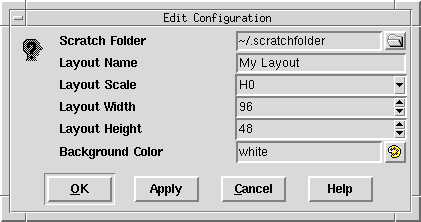
\includegraphics{EditConf.png}
\caption{Editing a set of preferences}
\label{fig:RC:EditConf}
\end{centering}
\end{figure}
The macro \lstinline=ReadConfiguration::ConfigurationType= can be used
to create an ensemble command to hold the preferences or configuration
options for your program.  This macro generates a Snit type that include
type methods to load, save, edit, and access preference or configuration
options. Typical code to use this macro is shown in
Listing~\ref{lst:RC:ConfigurationType} and the dialog box this macro
generates is shown in Figure~\ref{fig:RC:EditConf}.

